\subsection{Architecture overview}
As you know the main feature of the blockchain is its immutability. It means that once a smart contract (referred as contract from now on) is 
deployed, it's not possible to modify or update it. In order to update a contract you need to deploy 
a new contract on the blockchain.\\
In view of this fact and the proponent's request to develop upgradeable smart contracts, the architecture ideated and developed reflects these two aspects. As a matter of fact smart contracts in Soldino
are essentially of three types:
\begin{itemize}
	\item\textbf{Storage contract}: this type of contract isn't upgradeable because it's used
		to save all the critical data like products, orders, VAT movements;
	\item\textbf{Logic contract}: this type of contract implements the business logic. In addition
	a logic contract as a reference to its storage contract (e.g. UserLogic has a reference to UserStorage). This choice has been made to improve the security of the storage contract (it will be explained in \hyperlink{st}{\underline{section 7.2.2}});
	\item\textbf{Generic contract}: this type defines the contracts that aren't either logic nor storage.
	They are:
	\begin{itemize}
		\item\textbf{TokenCubit}: contract to implement the custom token ERC20 compliant \textit{Cubit};
		\item\textbf{ContractManager}: contract used to achieve simple upgradeablilty of the system;
		\item\textbf{Purchase}: contract to allows the user to buy several products with minimum number of transaction;
		\item\textbf{Owned} and \textbf{Authorizable}: contracts used for the system's security;
		\item\textbf{Migration}: contract provided by Truffle framework, it's used to deploy all contracts. 
	\end{itemize}
\end{itemize}

\begin{figure}[h]
	\centering
	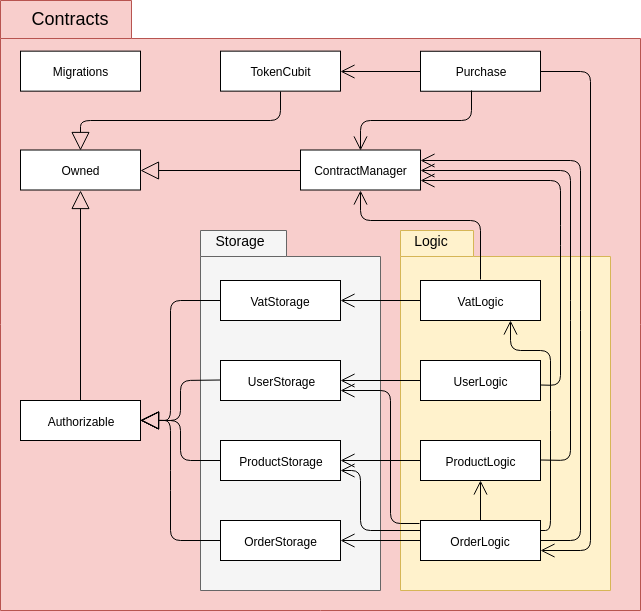
\includegraphics[scale=0.45]{res/images/architecture.png}
	\caption{Simplified class diagram of the contracts (state variables and methods are omitted)}
\end{figure}